\documentclass[12p, Times New Roman]{beamer}
\usepackage[utf8]{inputenc} 
\usepackage[croatian]{babel}
\usepackage{graphicx}
\usetheme{Ilmenau}

\title{Github vs Bitbucket}
\author{Luka Otović, Ivo Santini, Mauro Copetti}
\date{12.siječnja 2018.}
\institute{Tehnički fakultet Rijeka}


\begin{document}
	
	\frame{\titlepage}
	
	\begin{frame}     			% frame 1                                    
		\frametitle{GitHub}

		\begin{itemize}
			\item Tom Preston-Werner, Chris Wanstrath i PJ Hyett su ga objavili
		u travnju 2008. godine
			\item web-baziran je Git servis za kontrolu verzija
			\item koriste ga programeri u različite svrhe
		\end{itemize}

	\begin{figure}[h!]
		\begin{center}
			
\includegraphics[scale=0.10]{macka.png}
			\caption{Logo GitHub-a}
		\end{center}
	\end{figure}

	\end{frame}       

	\begin{frame}				% frame 2
		\frametitle{GitHub}
		\begin{itemize}
			\item najveći je domaćin izvornog koda u svijetu premašujući
	20 miljuna korisnika i 57 miljuna repozitorija
			\item vrijedi preko 2 milijarde USD

		\end{itemize}

		\begin{figure}[h!]
			\begin{center}
				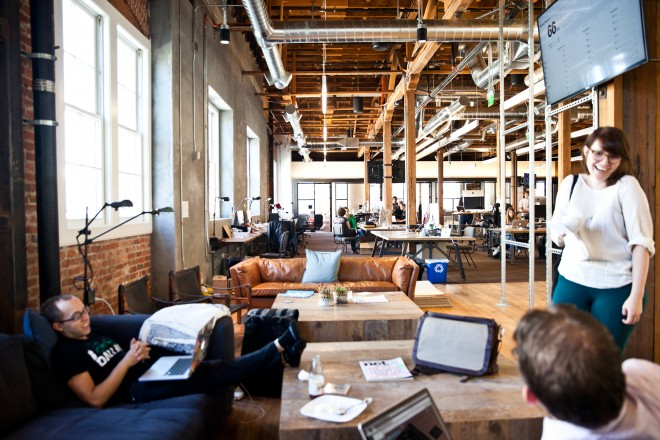
\includegraphics[scale=0.25]{headqgit.png}
				\caption{Sjedište GitHub-a}
			\end{center}
		\end{figure}


	\end{frame}



	\begin{frame}      			% frame 3        
		\frametitle{Bitbucket}

		\begin{itemize}
			\item osnovao ga je Jesper Nohr 2008. godine, a kasnije ga kupuje Atlassian
			\item web-baziran je Git i Mercurial servis za kontrolu verzija
			\item koristi se poput GitHub-a

		\end{itemize}

		\begin{figure}[h!]
			\begin{center}
				
\includegraphics[scale=0.04]{Bitbucket.png}
				\caption{Logo Bitbucket-a}
			\end{center}
		\end{figure}

	\end{frame}                



	\begin{frame}				% frame 4
		\begin{itemize}
			\item ima 5 milijuna korisnika
			\item vrijedi 160 milijuna USD

		\end{itemize}

		\begin{figure}[h!]
			\begin{center}
				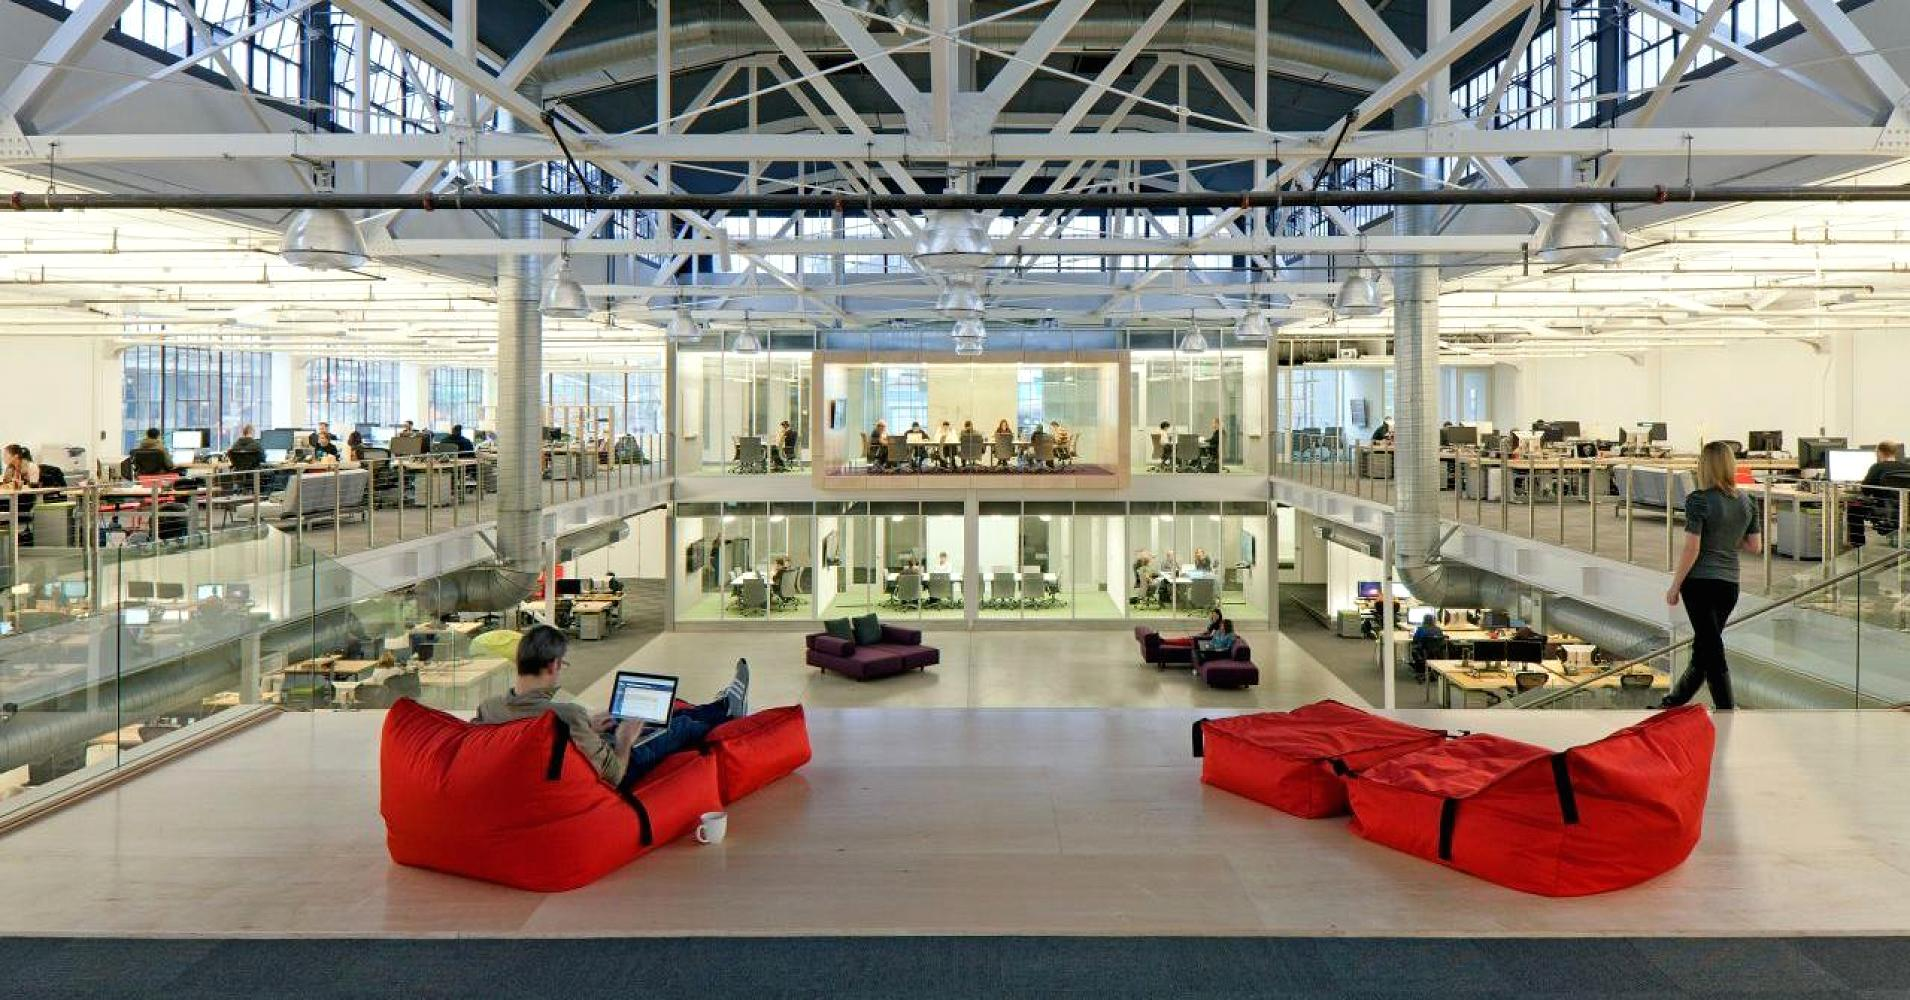
\includegraphics[scale=0.135]{headqbit.png}
				\caption{Sjedište Atlassian-a}
			\end{center}
		\end{figure}


	\end{frame}




	\begin{frame}    		    % frame 5
		\frametitle{GitHub vs Bitbucket}

		 \begin{figure}[h!]
			\begin{center}
				
\includegraphics[scale=0.34]{GVB.png}
			\end{center}
		\end{figure}
 


	\end{frame}                             

	\begin{frame}
		sliak velika za naslov `` SLIČNOSTI''

	\end{frame}


	\begin{frame} 			   % frame 6	
		\frametitle{Dizajn (GitHub)}
		
		\begin{figure}
			\begin{center}
				
\includegraphics[scale=0.1]{macka.png}
			\end{center}
		\end{figure}

	\end{frame}                              




	\begin{frame}
		\frametitle{Dizajn (Bitbucket)} 	% frame 7
		\begin{figure}
			\begin{center}
				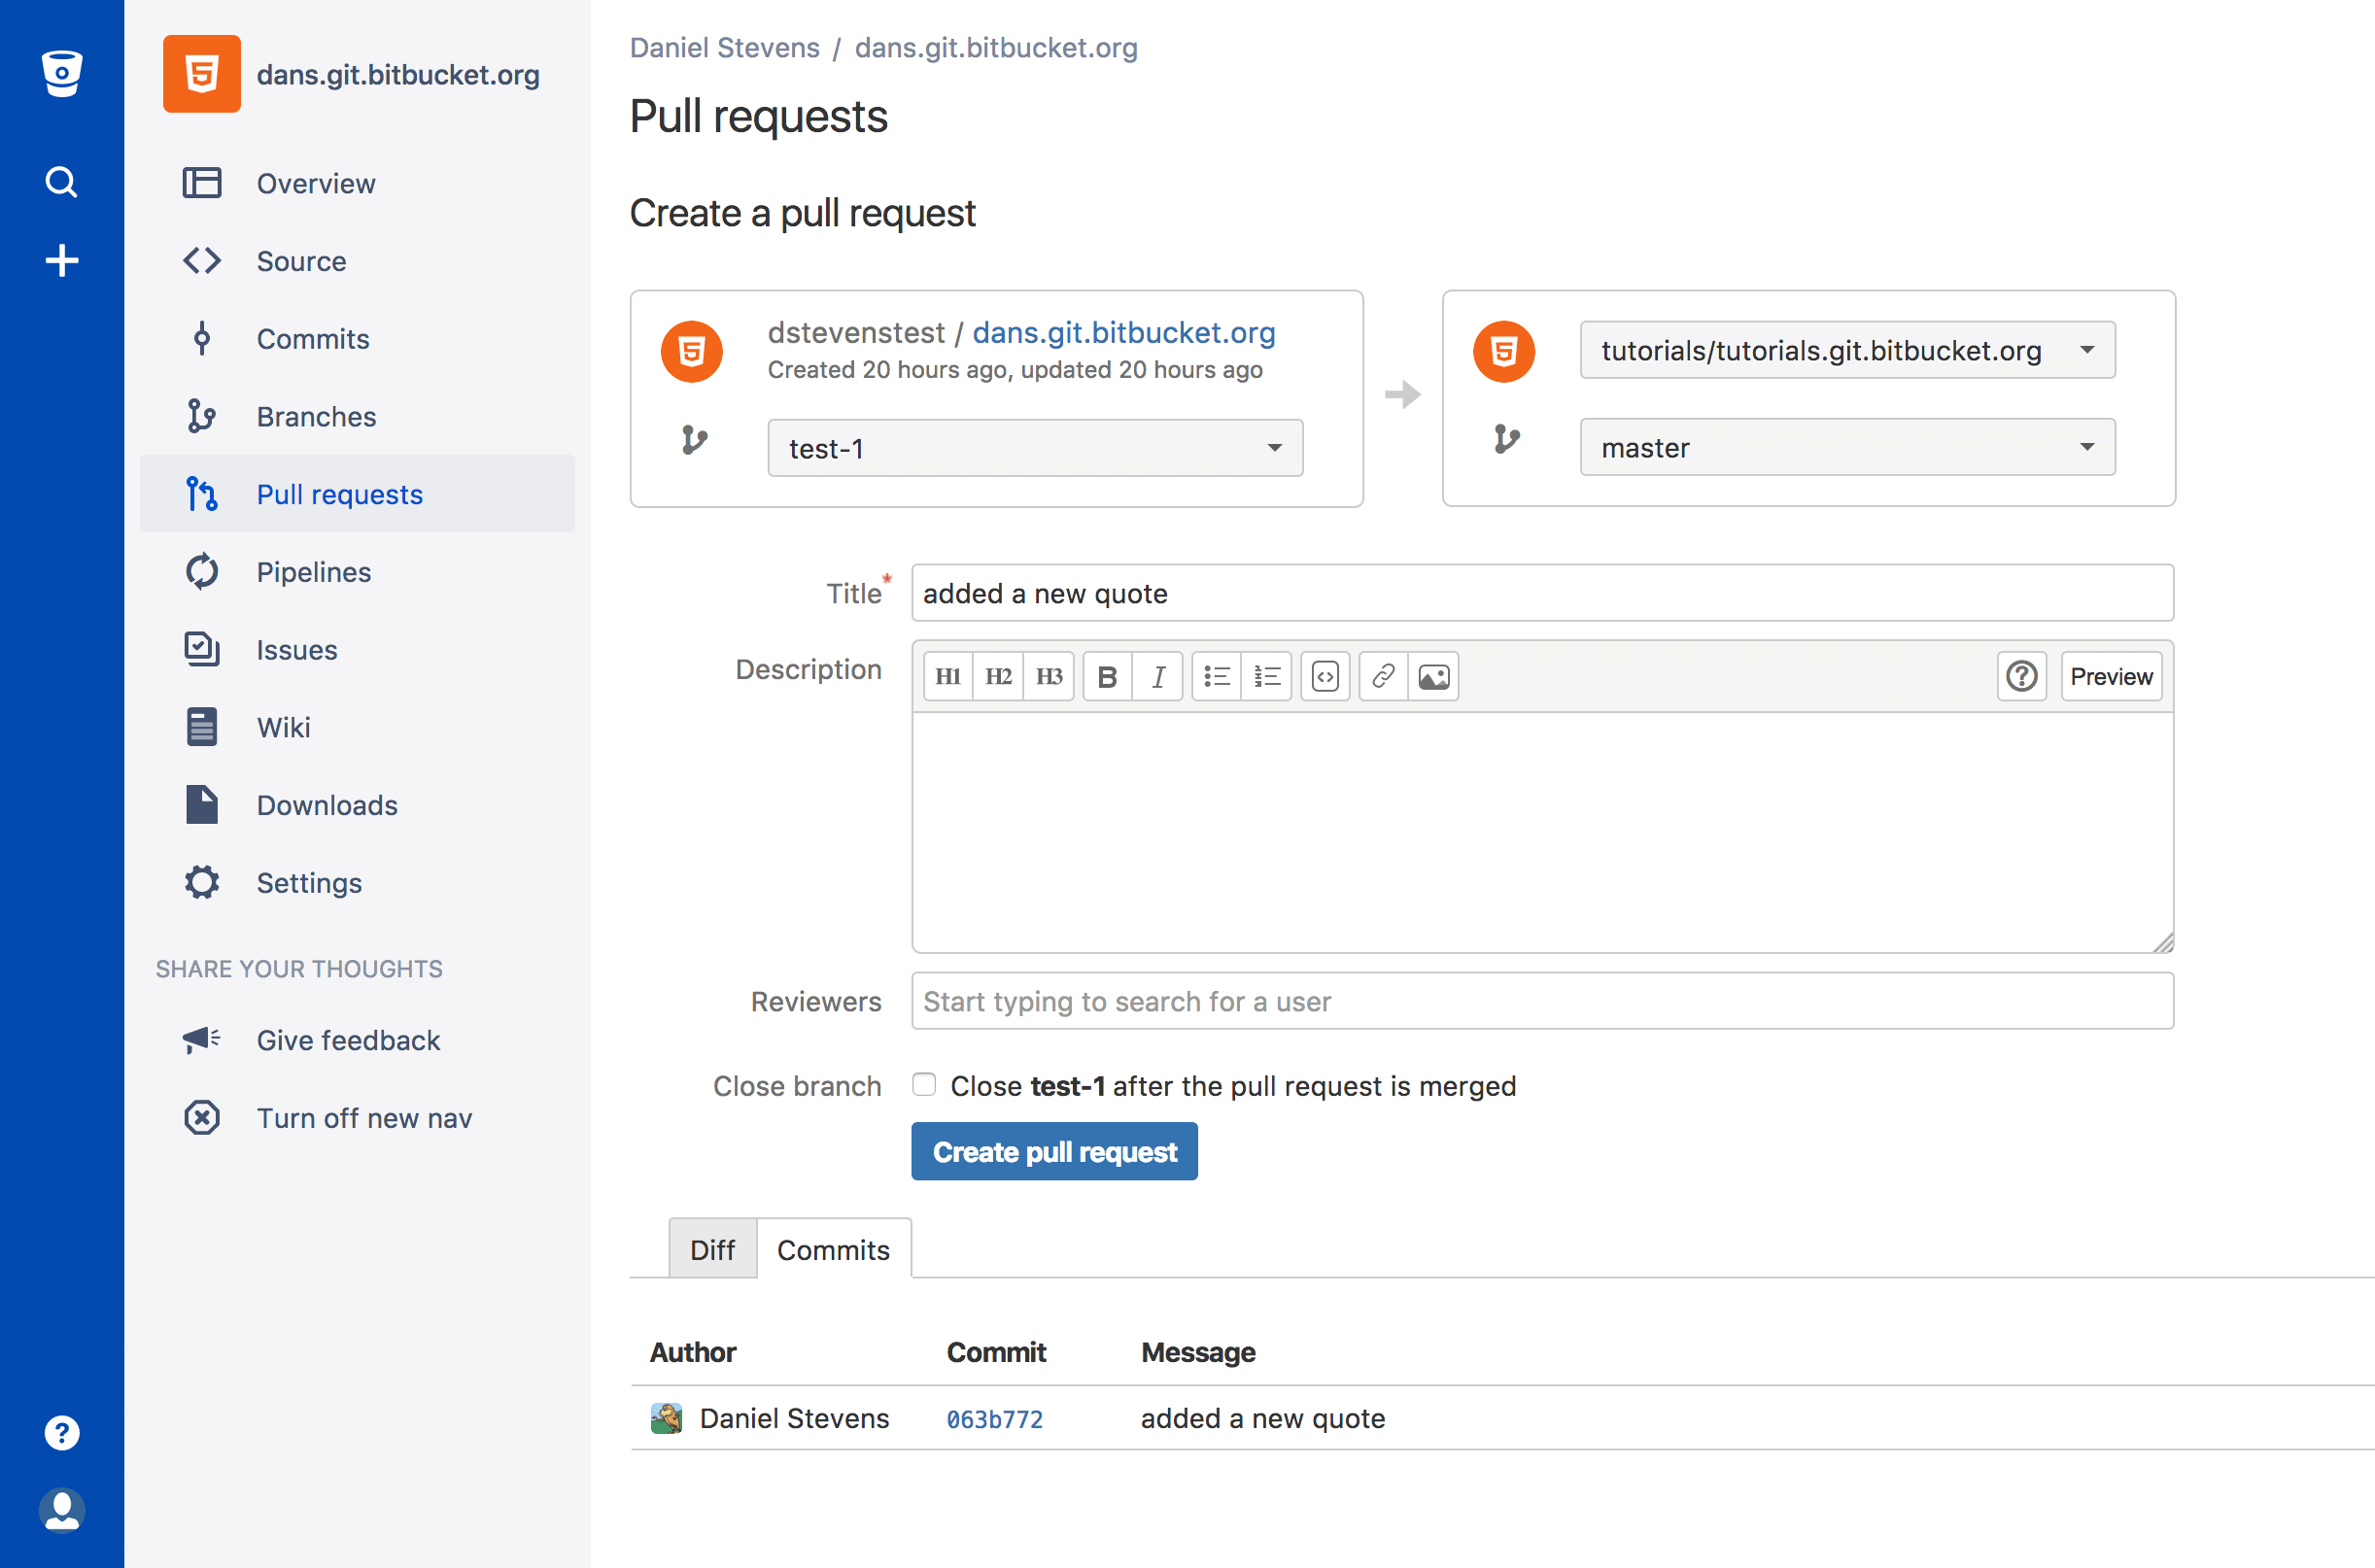
\includegraphics[scale=0.12]{Shot2.png}
			\end{center}
		\end{figure}

	\end{frame}

	\begin{frame}
		


	\end{frame}                           





	\begin{frame}


	\end{frame}

	\begin{frame}


	\end{frame}

	\begin{frame}


	\end{frame}

	\begin{frame}


	\end{frame}

	\begin{frame}


	\end{frame}

	\begin{frame}


	\end{frame}




\end{document}

